\chapter{Using an Internal Encoder}
\label{ch:using_internal_encoder}

% !!Restoring the original method with an internal encoder, !!mention that it was future work in the jazbec paper as well

\section{The Problem With External Encoders}

The \acs{DNI} experiment in \autoref{ch:semantic-encoder} revealed a fundamental
tension in the \citeauthor{jazbec_generative_2025} framework: by introducing an external
semantic encoder such as \acs{CLIP}, the method inadvertently displaced the epistemic
uncertainty signal away from the diffusion model and into the encoder itself. One can
bypass the posterior approximation entirely and still achieve near-identical filtering
performance, which goes
against the Bayesian motivation of the original framework. 
As formalized in \autoref{sec:formalize_dni_method}, 
the uncertainty score is proportional to the log Jacobian norms of the encoder, so the method effectively measures the encoder's local instability
rather than the diffusion model's posterior spread.

The natural fix is to use a feature representation that is \emph{internal} to the
diffusion model: semantically rich enough to avoid pixel-space pathologies, but directly
tied to the diffusion model's own learned manifold.

\section{Architecture of the ADM Model}
\label{sec:adm-architecture}

To understand why internal diffusion features can serve as a robust semantic representation, it is necessary to examine the architecture of the \acs{ADM} \parencite{dhariwal_diffusion_2021}. At its core, the \acs{ADM} relies on a U-Net architecture designed to take a noisy image as input and predict the added noise (or the denoised image) at the exact same spatial resolution. It achieves this through a symmetric pathway of encoding (downscaling) and decoding (upscaling) built primarily upon convolutional layers, augmented by attention mechanisms.

\paragraph{Convolutions and Local Features}
The foundational building block of the network is the convolutional layer. A convolution operation slides a small matrix of weights (a kernel or filter) across the input image or feature map, computing dot products at each spatial location. This allows the network to detect local patterns regardless of where they appear in the image. 
% In early layers, convolutions capture basic structural elements like edges and textures; in deeper layers, they combine these elements to represent complex objects and semantic concepts.

\paragraph{The Encoder and Downscaling}
The first half of the U-Net is the encoder, which progressively compresses the spatial dimensions of the input while expanding its feature depth. This downscaling is achieved through strided convolutions or pooling operations, which reduce the width and height of the feature maps (e.g., from $128 \times 128$ to $64\times 64$). As spatial resolution decreases, the number of feature channels ($C_\ell$) increases. This process forces the network to discard fine-grained, pixel-level spatial details and instead encode, high-level semantic information. The network reaches its most compressed state at the ``bottleneck'', where the spatial dimensions are at their minimum and the channel count is at its maximum.

% These attention layers allow the model to weigh the importance of all spatial locations relative to one another simultaneously, 
% combining the local feature extraction of convolutional layers with the global semantic awareness of Transformers.

\paragraph{The Decoder and Upscaling.}
The second half of the U-Net is the decoder, which is responsible for projecting the compressed, abstract representations back into the original pixel space. It achieves this through upscaling operations, progressively increasing spatial resolution while decreasing the channel count. To ensure that fine spatial details lost during downscaling are retained, the U-Net employs ``skip connections'' that directly concatenate feature maps from the encoder to their corresponding layers in the decoder.

\paragraph{Global Context via Attention}
While convolutions are highly effective at capturing local features, they struggle with long range dependencies (e.g. understanding how a feature in the top left corner of an image relates to one in the bottom-right). To address this, the \acs{ADM} U-Net intersperses attention layers throughout its architecture, particularly at lower resolutions ($8 \times 8$ to $32 \times 32$). 
% \vspace{1em}
% \textit{(You can then transition smoothly into your modified Section 2, where you explain exactly why you target the start of this decoder phase.)}
% \vspace{1em}

% \section{UNet Bottleneck Features}
% \label{sec:bottleneck}

% The \acs{ADM} UNet produces intermediate feature maps throughout its decoder blocks (\texttt{output_blocks}). Because the network's understanding of the image is most semantically concentrated at the lowest resolutions, we target the features generated immediately after the bottleneck. At this stage, the spatial resolution is low and the channel count is high, providing a compact, highly descriptive representation of the image manifold without requiring any external encoder.

% We extract these features using PyTorch forward hooks... *(continue with your original text)*

\section{UNet Features Uncertainty}
\label{sec:bottleneck}

The \acs{ADM} UNet produces intermediate feature maps at its decoder blocks
(\texttt{output\_blocks}, \autoref{tab:adm-unet-decoder}). Near the bottleneck, spatial resolution is low and channel count $C_\ell$ is high, giving a compact, semantically rich representation without any external encoder. We extract these features using PyTorch forward hooks: for each forward pass,
the hook applies global average pooling (\texttt{F.adaptive\_avg\_pool2d}) to collapse
spatial dimensions, yielding a $C_\ell$-dimensional vector per image. Hooks are
registered once before the weight-draw loop and removed afterwards, leaving the network
unaltered.

% \paragraph{Layer selection (WIP)} Early decoder blocks are preferred for two reasons. First,
% they are closest to the bottleneck and therefore most semantically rich. 

% Second, as one moves further into the decoder the spatial resolution grows, rapidly increasing $C_\ell$
% and with it the variance of the entropy estimator which is problematic given only
% $M = 6$ samples. 
% The exact channel dimensions should be confirmed at runtime via \texttt{dict(model.named\_modules())}.

\begin{table}[!htbp]
\centering
\caption{ADM UNet \texttt{output\_blocks} structure for ImageNet $128\times128$,
         extracted from \texttt{model.named\_modules()}.
         Each output block is made out of a sequence of submodules.
         % The \texttt{.2} sub-block in blocks 2, 5, 8, and 11 is the up/downsampling
         % ResBlock. Blocks 9--14 operate without attention.
         We assign indexes to sub-modules inside each block (e.g. \texttt{0.Res} in \texttt{output\_block.0} will be identified as \texttt{output\_blocks.0.0}, the first sub-module in the first block)}
\label{tab:adm-unet-decoder}
\begin{tabular}{llcc}
\toprule
\textbf{Block} $\downarrow$ & \textbf{Sub-modules} $\rightarrow$ & \textbf{Spatial res.} & \textbf{Channels}\\
\midrule
output\_blocks.0  & 0.Res + 1.Attention & $8\times8$     & 1024  \\
output\_blocks.1  & 0.Res + 1.Attention & $8\times8$     & 1024  \\
output\_blocks.2  & 0.Res + 1.Attention + Upsample   & $8\times8$     & 1024 \\
\midrule
output\_blocks.3  & 0.Res + 1.Attention & $16\times16$   & 512 \\
output\_blocks.4  & 0.Res + 1.Attention & $16\times16$   & 512 \\
output\_blocks.5  & 0.Res + 1.Attention + Upsample   & $16\times16$   & 512 \\
\midrule
\dots & \dots & \dots & \dots\\
output\_blocks.14 & 0.Res & $128\times128$ & 256  \\
\bottomrule
\end{tabular}
\end{table}

% \paragraph{Timestep selection} Features are captured at the following \acs{DDIM} loop indices:
% \begin{equation}
%     t \in \{45, 40, 35, 30, 25, 20, 15, 10, 5\}
% \end{equation}

\paragraph{Uncertainty computation} For a given (layer, timestep) pair, the
$C_\ell$-dimensional feature vectors from all $\mathrm{M}$ draws are stacked into an
$(N, \mathrm{M}, C_\ell)$ tensor (with $N$ the number of images generated per model). Per-image entropy is computed under a diagonally approximated Gaussian:
% \begin{equation}
%     U(\mathbf{x}) = \frac{1}{2} \sum_{k=1}^{C_\ell} \ln\!\left(\hat{\sigma}^2_{\phi,k}
%     \right) + \frac{C_\ell}{2}\ln(2\pi e).
%     \label{eq:internal-entropy}
% \end{equation}
\begin{equation}
    U(\mathbf{x}) = \frac{1}{2} \sum_{k=1}^{C_\ell} \ln\!\left(\hat{\sigma}^2_{\phi,k}
    \right) + const
    \label{eq:internal-entropy}
\end{equation}

Where $\hat{\sigma}^2_{\phi,k}$ is the empirical variance computed from the k-th dimension of the $C_\ell$ sized feature vector across the $\mathrm{M}$ models outputs.

\subsection{The Experiment}
\label{sub:internal-enc-abla-exp}

We are going to conduct an ablation to find the best sub-module (\texttt{output\_blocks.i.j} \autoref{tab:adm-unet-decoder}) and timestep $t$ at which to extract the feature maps in order to minimize the \acs{HPS} \acs{AURC} metric. 

We use the \acs{HPS} \acs{AURC} metric because it is much faster to compute than the \acs{FPR} metrics (\autoref{sub:adv_hps_eval_speed}) and gives a single number as output which makes the comparison easy. 

Once we find the best combination, we compare it to results obtained with the original \acs{CLIP} based method on both the \acs{HPS} \acs{AURC} and the \acs{FPR} metrics.

We will go through the layers and sub-modules contained in \texttt{output\_block.i.j} $i \in [0,\dots 5]$ and timesteps $t \in \{45,40,\dots,5\}$ out of 50 \acs{DDIM} steps, with $0$ being the final output $x_0$ and $50$ being the starting noise $z$.
(These are not raw diffusion timesteps as in \acs{DDPM}: each index in a 50-step uniform schedule
maps to a specific $t$ determined by the \acs{DDIM} skip schedule (\autoref{sec:bg_diffusion})).

\subsection{Results}

First, for each sub-module we compute the \acs{HPS} \acs{AURC} for each $t$ and report the best value for each sub-module. We get the following results:

\begin{lstlisting}[frame=tb,caption={best AURC(t) per sub-module},label=lst:useless]
output_blocks.0.0 best AURC: 11.76 at t=5 <--
output_blocks.0.1 best AURC: 11.82 at t=5
output_blocks.1.0 best AURC: 11.87 at t=5
output_blocks.1.1 best AURC: 11.74 at t=5 <--
output_blocks.2.0 best AURC: 11.96 at t=5
output_blocks.2.1 best AURC: 11.86 at t=5
output_blocks.2.2 best AURC: 11.87 at t=5
output_blocks.3.0 best AURC: 11.98 at t=5
output_blocks.3.1 best AURC: 11.95 at t=5
output_blocks.4.0 best AURC: 12.13 at t=5
output_blocks.4.1 best AURC: 12.09 at t=5
output_blocks.5.0 best AURC: 12.22 at t=5
output_blocks.5.1 best AURC: 12.12 at t=5
output_blocks.5.2 best AURC: 12.16 at t=5
\end{lstlisting}

The two best layers are \texttt{output\_block.1.1} (AttentionBlock) followed closely by \texttt{output\_block.0.1} (AttentionBlock). The general trend is that the higher (block id) we go in the decoder, the worse the \acs{HPS} \acs{AURC} gets. The minimum \acs{AURC} is always obtained at the minimum timestep $t=5$ (closest fully denoised to final output).

\begin{figure}[!htbp]
    \centering
    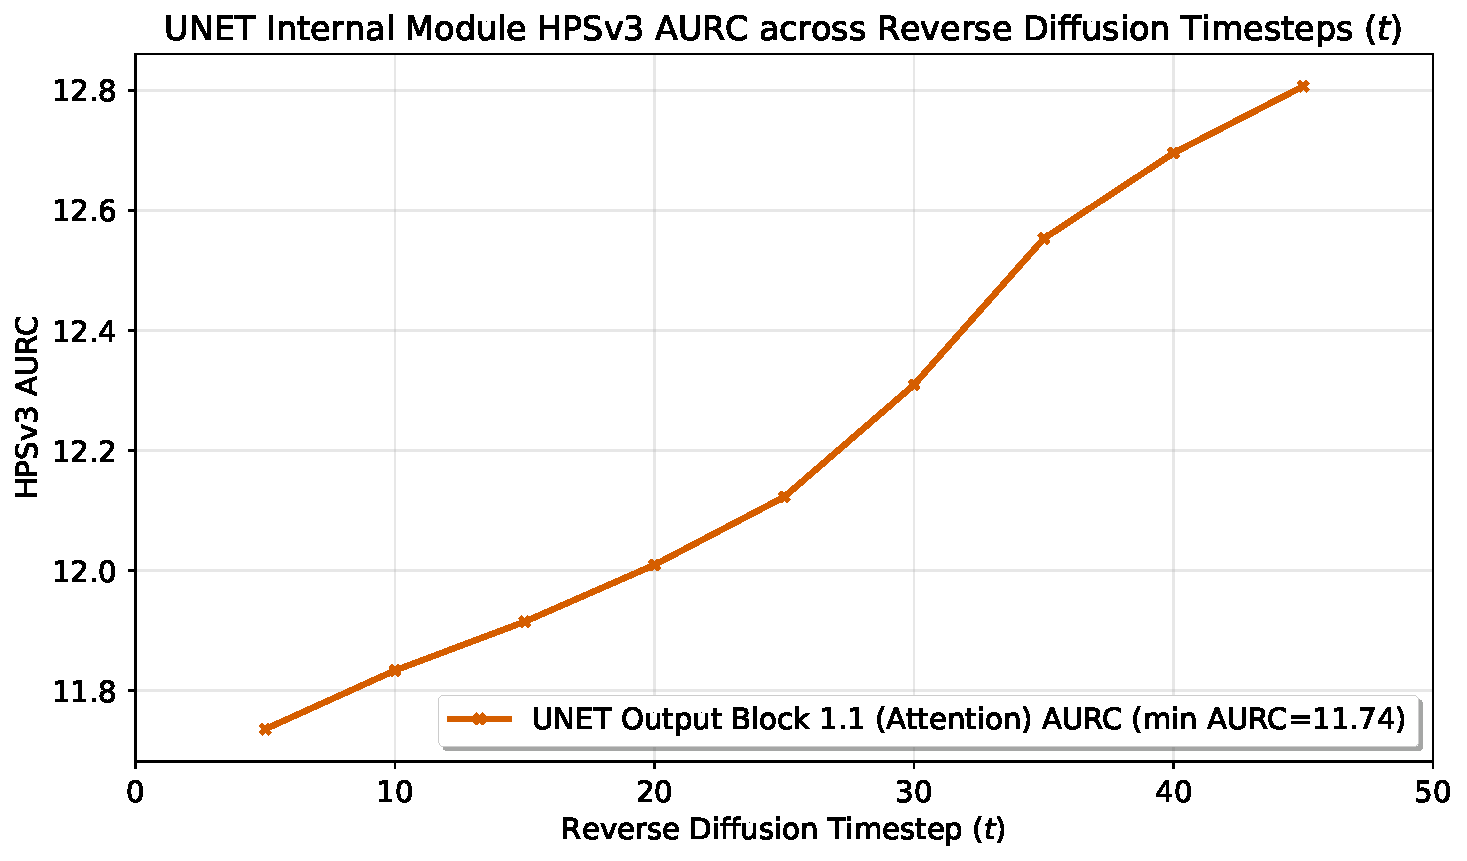
\includegraphics[width=0.9\linewidth]{figures/internal/aurc_unet_t.pdf}
    \caption{\acs{HPS} \acs{AURC} across $t$ for \texttt{output\_block.1.1}}
    \label{fig:aurc_unet_t}
\end{figure}


We can take a closer look at the \acs{HPS} \acs{AURC} for \texttt{output\_block.1.1} at each $t$ in \autoref{fig:aurc_unet_t}. It seems like going down to $t=0$ should yield even better results.

\begin{tcolorbox}[colback=orange!10!white,colframe=orange!50!black,sharp corners]
The observation that $t=0$ should be the best timestep at which to compute uncertainty helps justify \cite{jazbec_generative_2025} approach to only track generative uncertainty at the last step of the reverse diffusion process instead of during whole process (\autoref{sub:gu_theory_issue_multi_step}).
\end{tcolorbox}

\paragraph{UNET vs CLIP on the AURC HPSv3 metric}
Let's now compare the UNET Internal Sub-Module \texttt{output\_block.1.1} at $t=5$ to the \acs{CLIP} external feature extractor. We can see on \autoref{fig:aurc_clip_unet} that despite not being as good as \acs{CLIP} we manage to remain surprisingly close in the lower rejection rates.

\begin{figure}[!htbp]
    \centering
    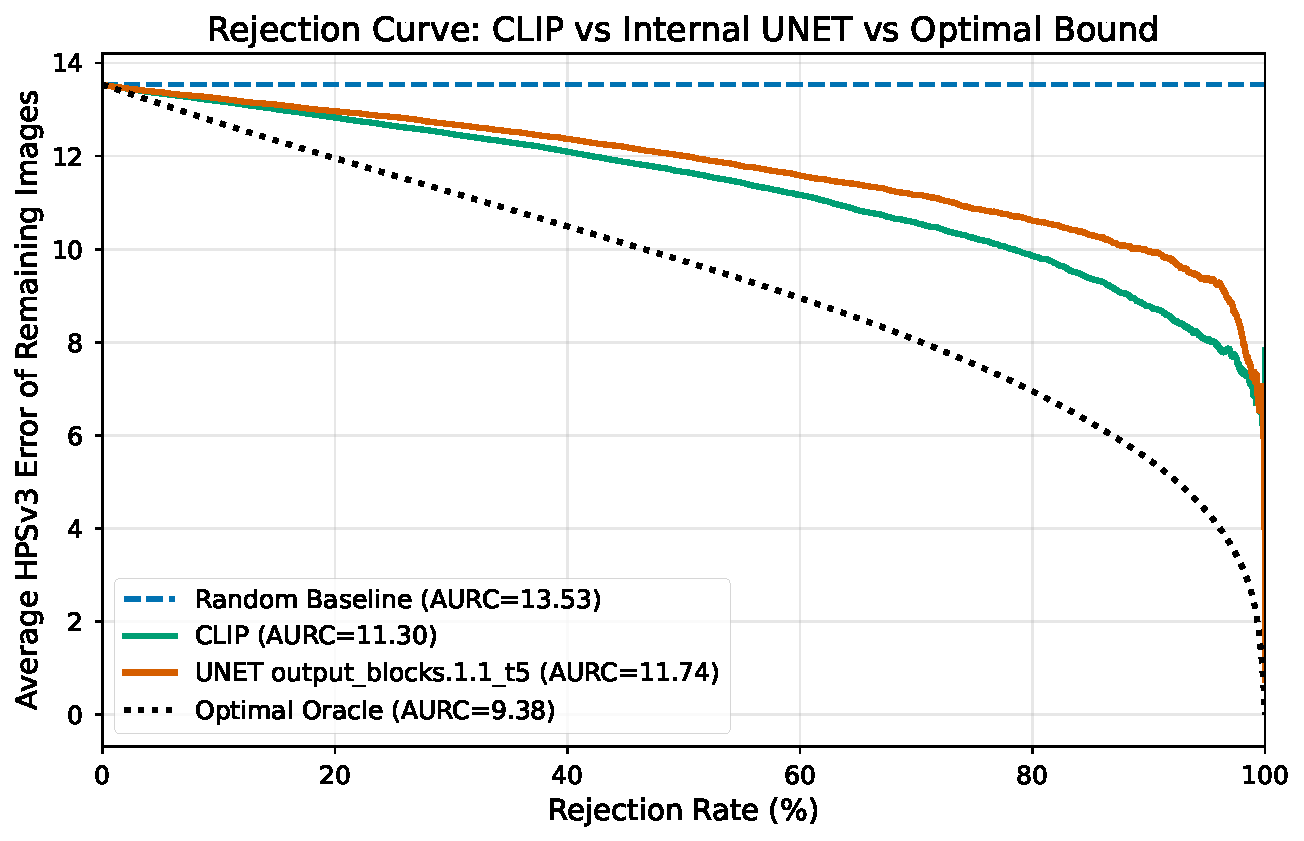
\includegraphics[width=0.9\linewidth]{figures/internal/aurc_clip_unet.pdf}
    \caption{HPSv3 Rejection Curve comparing the uncertainty we get when using the \acs{CLIP} encoder against the Internal UNET encoder}
    \label{fig:aurc_clip_unet}
\end{figure}

It's not so surprising that \acs{CLIP} works better at filtering for an \acs{HPS} metric.
HPSv3 and \acs{CLIP} were both trained on a dataset of natural images that goes beyond what ImageNet contains. Whereas our Internal UNET encoder from \acs{ADM} was only trained on ImageNet. As we've seen in \autoref{ch:semantic-encoder}, the uncertainty score is largely influenced by the training manifold of the encoder, \acs{CLIP} having a training manifold closer to the HPSv3 model than \acs{ADM} gives \acs{CLIP} an advantage over the Internal UNET on the HPSv3 metric specifically.

\paragraph{UNET vs CLIP on the FID, Precision and Recall metrics}
Let's now compare \acs{CLIP} and UNET Internal on the \acs{FPR} metrics \autoref{sec:inception_metrics}:

FID for instance is comparing the statistical distribution of a large subset of the reference ImageNet dataset with a subset of the \acs{ADM} generated images (The subset is created by removing the highest uncertainty images first).
We expect Internal UNET to perform better on those metrics since it is made to filter out images that are out of the training manifold of \acs{ADM} itself.
\autoref{fig:unet_vs_clip_fpr} mostly confirms this: 
\begin{itemize}
    \item \acs{FID}: Remains lower than \acs{CLIP} for longer, meaning the UNET uncertainty understands better what is not a valid sample with respect to the ImageNet dataset statistical distribution.
    \item \emph{Recall}: Remains much higher, we manage to maintain more diversity during the filtering.
    \item \emph{Precision}: The cost of higher recall is usually linked to a lower precision, which is also the case here, but we manage to not lose too much here.
\end{itemize}

\begin{figure}[!htbp]
    \centering
    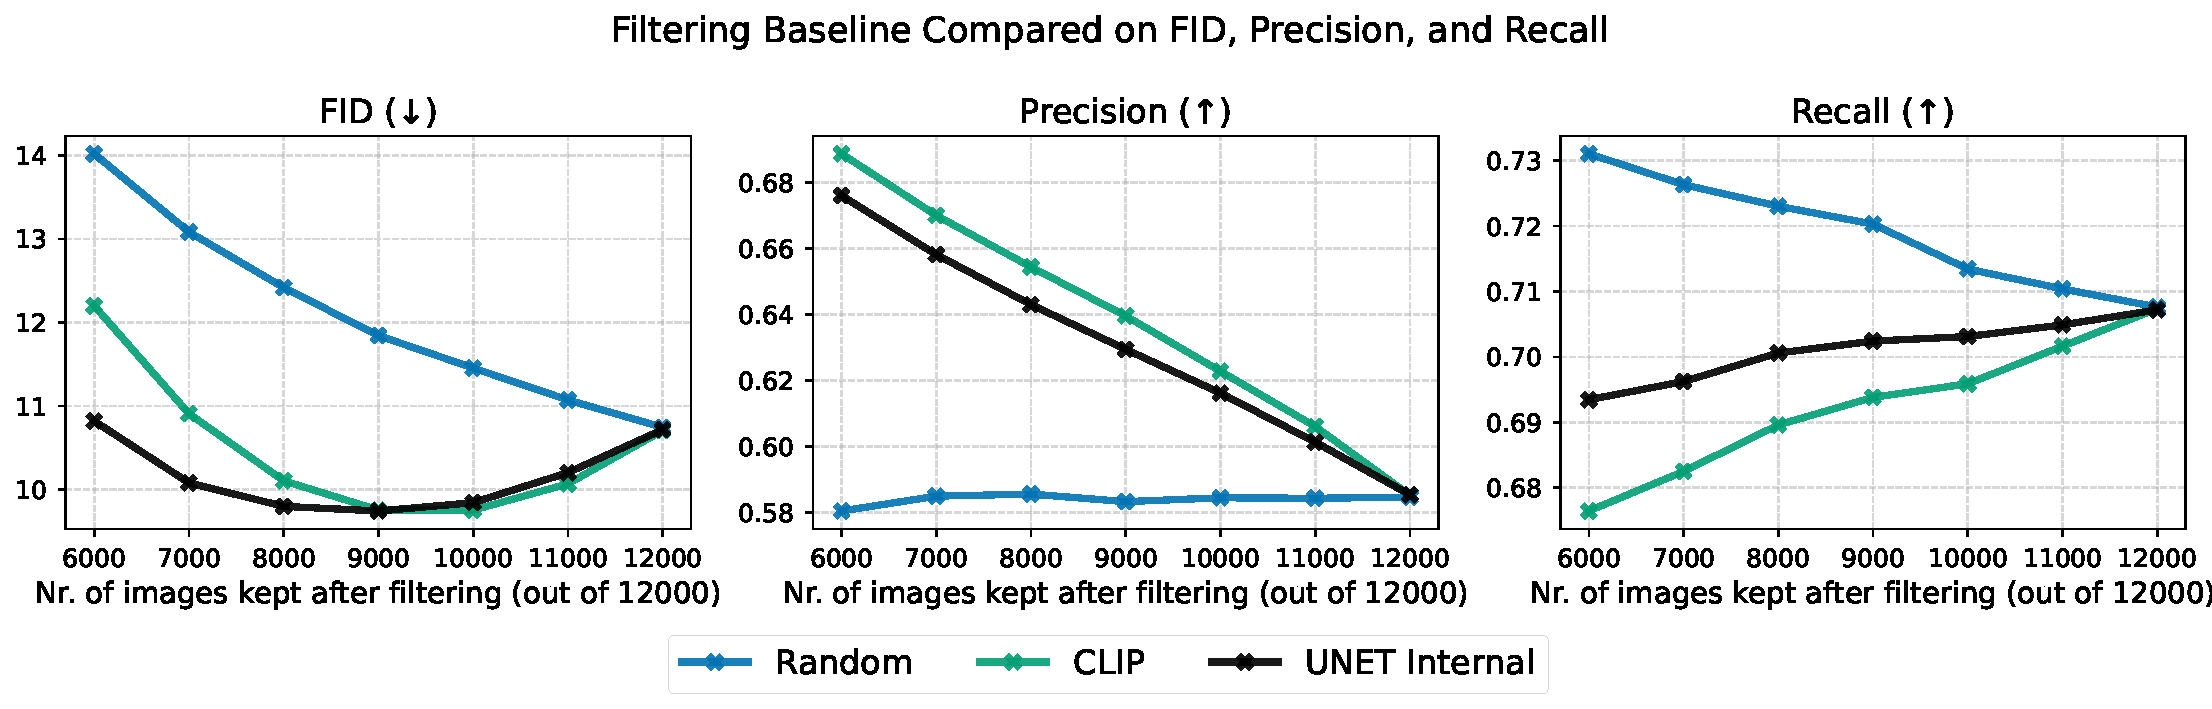
\includegraphics[width=0.98\linewidth]{figures/internal/unet_vs_clip_fpr.pdf}
    \caption{Comparing the uncertainty we get when using the CLIP encoder against the Internal UNET encoder on the \acs{FPR} metrics. \warning as previously explained in \autoref{sub:problems_inception}, the \texttt{random} baseline should be flat, it's growth roughly represents the bias induced by reducing the number of samples that affects all filtering baselines}
    \label{fig:unet_vs_clip_fpr}
\end{figure}


\subsection{Relation to Prior Work}
\label{sec:internal_features_prior_work}

% The principle behind the \acs{DNI} and the internal encoder sits close to several existing lines of work.

% The internal-encoder direction proposed above, and its pairing with \acs{DNI}, sits close to several existing lines of work. 

% We position both here, as a continuation of the \acs{DNI} experiment of \autoref{ch:semantic-encoder}, since the relevant neighbors span that chapter and this one. In each case the novelty lies less in the mechanism than in how it is used.

Using internal layers of a diffusion model as semantic representations is not a new idea, \cite{baranchuk_label-efficient_2022} argue that those layers can ``potentially be used as image representations for downstream tasks'' in their case they demonstrate their claim with a segmentation downstream task. 

More recently, \cite{luo_diffusion_2024} go over the same idea but also explore how semantic content of the features spread across layers and timesteps. In our \autoref{sub:internal-enc-abla-exp} ablation, we only try to find the best combination but leave the question of whether multiple layers/timesteps can be combined for future work.

\subsection{Internal Encoder Filtering vs Classifier Guidance}

In \autoref{ch:classifier} we found that adding classifier guidance to the \acs{ADM} reduced the FID down further than any filtering method. 
By using the internal encoder however, we manage to keep the FID lower during a much larger part of the filtering process \autoref{fig:unet_vs_clip_fpr}. Although we don't get as low as the classifier guidance, taking into account the bias (represented by the \texttt{random} baseline) induced by reducing the number of samples (\autoref{sub:show_n_inception_problem}), we can say that the internal encoder filtering is close to the classifier guidance results on the \acs{FID} metric. 

\subsection{Future Work to Improve the Internal Encoder}


\paragraph{The Last Layer Perturbation}
One important caveat that could further discredit the heavily approximated Bayesian posterior's role in the uncertainty score: only the last layer of the \acs{ADM} model is perturbed by the
\acs{LLLA}. The variance in intermediate features is therefore entirely a downstream consequence of that last-layer perturbation propagated through the forward pass, not a direct measure of uncertainty in those layers. Either this was enough to capture meaningful epistemic uncertainty. Or as previously suggested, the Bayesian model is over-approximated and acts more like a random noise generation similar to the \acs{DNI} method than a proper Bayesian uncertainty signal which could be enough to get meaningful results and further motivates trying \acs{DNI} on the internal encoder.

\paragraph{Feature Extraction}

The internal feature extraction method itself could be improved in a couple of ways. 

First, we've not measured the correlation between the uncertainty measurement taken at different timesteps and sub-modules, if they happen to complement each other, it should be possible to combine them together and get better results.

Then, we've used a rather simple average pooling of $8\times8, 16 \times 16, \dots$ feature maps to get our feature vector. Doing so loses a lot of information and is probably not the best method.

Finally, results suggested that $t=0$ would be an even ``better'' timestep at which to compute uncertainty w.r.t. the \acs{HPS} \acs{AURC} metric.

% \paragraph{Cross-cutting directions}
% Three further directions span this chapter and \autoref{ch:semantic-encoder}, so we develop them in the Conclusion rather than duplicate them here (\autoref{ch:conclusion}): pairing this internal encoder with \acs{DNI} to obtain a cheap, model-intrinsic filter, the direction we would pursue first; recovering a useful Bayesian signal through a stronger posterior approximation \parencite{gegenfurtner_reducing_2026, gupta_quantifying_2026} able to survive the encoder bottleneck; and clarifying how the local-sensitivity signal \acs{DNI} measures relates to genuine weight-space uncertainty, within a single basin (\acs{LLLA}) and across basins (\acs{DE}), as studied on the Toy model in \autoref{ch:toy_exp_posterior}.

\subsection{Discussion around the Bayesian Method Role}

Up until now we have argued for the heavily approximated Bayesian posterior's role to be useful for the \textit{Toy Model} and not for the \acs{ADM}. Here we argue for the Bayesian posterior's role to be useful for the \acs{ADM} as well.

From our observations, when we sample the Bayesian posterior predictive, we get a distribution of images that do have \textbf{structural} changes (look closer to the images generated from the posterior in \autoref{fig:pipeline_posterior_to_vector}). This is a good sign that the Bayesian posterior is indeed capturing some epistemic uncertainty in the model's weights. 

What we believe could have happened in \autoref{ch:semantic-encoder} is that the \acs{CLIP} encoder was not able to ``understand'' those structural changes, the perturbation being noise or slight structural changes did not change much for the \acs{CLIP} encoder and therefore the uncertainty score was not able to capture the epistemic uncertainty in the model's weights. The internal encoder on the other hand is able to capture those structural changes and would therefore reflect the epistemic uncertainty in the model's weights better than \acs{CLIP}.

\section{Conclusion}

The Bayesian Framework \acs{LLLA} with an internal encoder significantly outperforms every other filtering metrics we've tried so far when it comes to the \acs{FPR} metrics (representing how close the filtered image dataset is to the reference distribution). On the other hand, the \acs{CLIP} external encoder is still better on the \acs{HPS} \acs{AURC}, likely because of the training manifold of \acs{CLIP} being closer to HPSv3 than the \acs{ADM}.

The quality of the internal encoder could still be improved further. But the main question is whether the Bayesian framework is actually providing value to the uncertainty score in this internal encoder context or if once again \acs{DNI} could get close to the same results with a much cheaper computation cost. We believe that any semantic encoder probed with \acs{DNI} should be able to detect out of training manifold samples and therefore be a good filtering metric. 
But because the internal encoder should understand structural changes induced by the Bayesian posterior predictive, it is likely that \acs{LLLA} will be better than \acs{DNI} in this context. 



% The internal encoder derived in this chapter builds on a now-large body of work showing that a diffusion U-Net's intermediate activations form a rich semantic representation, exploited for segmentation, semantic correspondence, and other discriminative downstream tasks.
% TODO add citations: Baranchuk et al. (DDPM-Seg), Tang et al. (DIFT, arXiv 2306.03881), Luo et al. (Diffusion Hyperfeatures, arXiv 2305.14334), survey arXiv 2407.00783
% What distinguishes our use is the task: rather than transferring these features to an external discriminative problem on real images, we turn them inward, using the model's own representation to score the quality and off-manifold instability of its \textit{own} generations. Notably, an intrinsic feature extractor of this kind was itself flagged as future work by \cite{jazbec_generative_2025}, so our internal encoder is best read as an attributed extension of their framework rather than a departure from it.